\documentclass[11pt]{article}[]
\usepackage[a4paper, total={6.4in,9.2in}]{geometry}
\usepackage[pdftex]{graphicx}
\usepackage{amsfonts}
\usepackage{amsthm}
\usepackage{amssymb}
\usepackage{amsmath}
\usepackage{bibentry}
\usepackage{hyperref}

\begin{document}	

\begin{center} \Large \textbf{Model of phosphate transport in the cell}\\ \vskip 2mm
\normalsize {Kira M. D\"usterwald, \today}
\end{center} 

\normalsize

Phosphate is an important intracellular molecule required for the synthesis of nucleic acids. However, the inclusion in the cell and effects on other ions are not well understood. Here, we extend a pump-leak model for chloride homeostasis in neurons to incorporate a sodium-phosphate (Na-Pi) co-transporter \cite{Dusterwald2018}. The model predicts hyperpolarisation of the membrane potential and increases in intracellular potassium and sodium in response to phosphate influx. Predicted theoretical results can help to understand experimental results and suggest confirmatory experiments.

\section{Methodology}

We assume an infinite bath setting in a model including the ATPase pump (which can be dynamic, dependent on the sodium gradient, or static), Na\textsuperscript{+}, Cl\textsuperscript{-} and K\textsuperscript{+} ion fluxes, a potassium-chloride co-transporter, and dynamic cellular volume \cite{Dusterwald2018}. The Na-Pi transporter is modeled as an electrogenic pump harnessing the sodium gradient \cite{Levi2019}. That is,
\begin{equation}
J_{Na-Pi} = g_{Na-Pi} (E_{Na}-V_m)
\end{equation}
Usually, the sodium reversal potential $E_{Na}$ is greater than the membrane reversal potential $V_m$, so $J_{Na-Pi}$ is positive. In this setting, we expect sodium to enter the cell using the passive gradient, co-transporting phosphate ions through the selectively-permeable symporter. Because phosphate has a valency of -3, charge neutrality is guaranteed by transporting 3 sodium ions for every phosphate ion \cite{Levi2019}. Then the differential equation describing sodium evolves:
\begin{equation}
\frac{d[Na^+]_i}{dt}=-\frac{A_m}{F}\big(g_{Na}(V_m-E_{Na})+3J_p\mathbf{-3J_{Na-Pi}}\big)
\end{equation}

Phosphate is assumed only to be able to cross the cell membrane through the Na-Pi transporter. Otherwise, it is part of the group of impermeant anions. When the intracellular component of phosphate increases, either the number (mols) of impermeant anions is increased, or the phosphate is incorporated immediately into an existing impermeant anion (nucleic acid, e.g. DNA) while the number of impermeant anions stays the same \cite{Engstrom1983}, i.e., 
\begin{equation}
\text{Pi}+\text{DNA} \rightarrow \text{DNA-Pi}
\end{equation}

In the case that phosphate is not incorporated into DNA, the concentration and valency or average charge $z$ of impermeant anions $X$ are adjusted as follows:
\begin{eqnarray}
\frac{d[X^z]_i}{dt} & = d[X^z]_i(t+1) - d[X^z]_i (t) = -\frac{A_m}{F} \big(\mathbf{J_{Na-Pi}}\big) \\
z(t+1) &= \frac{z(t)*[X^z]_i (t) -3*\big(d[X^z]_i(t+1) - d[X^z]_i (t)\big)}{[X^z]_i(t+1)}
\end{eqnarray}

In the case that phosphate is not incorporated, $[X^z]_i$ does not change from phosphate influx directly, and $z$ is updated according to:
\begin{equation}
z(t+1) = \frac{z(t)*[X^z]_i (t) -3*-\frac{A_m}{F} \big(\mathbf{J_{Na-Pi}}\big)}{[X^z]_i(t)}
\end{equation}
Volume updates and resultant changes to concentrations are calculated after the above steps.

\section{Results}

The sodium-phosphate transporter was activated for a short period of time between 250s - 1750s in all experiments, using the same conductance $g_{Na-Pi}$. A steady state is not reached during the activation time period. Sodium and phosphate (impermeant anions) flux into the cell during activation. The interim values for all simulations are shown in the Appendix, \ref{app}.

\subsection{Steady state: Decreased ionic potential equilibria and increased volume}

We compare phosphate entering the cell but remaining separate from DNA (Figure \ref{f1}), and entering the cell and combining with DNA (Figure \ref{f2}) with dynamic (cubic dependence on sodium concentration) and static (constant) ATPase rates. At steady state after the Na-Pi transporter is switched off, all models equilibrate with relative decreases in $E_{Na},E_K,E_{Cl}$ and $V_m$ compared to baseline (Figure \ref{f1},f{2}, top and middle panels). These homeostatic changes are expected, since $z$ has decreased \cite{Dusterwald2018}.

Because there are more intracellular molecules from the 3 sodium: 1 phosphate influx, volume of the cell increases, and there is a relative decrease in the concentration of impermeant anions, regardless of whether phosphate is incorporated in DNA or not. The change is nonetheless greater when phosphate is incorporated in DNA, since no new impermeant anion mols are added to the cell (Figure \ref{f2}, bottom panels).

\begin{figure}[h]
\centering A  \hskip 80mm B \\
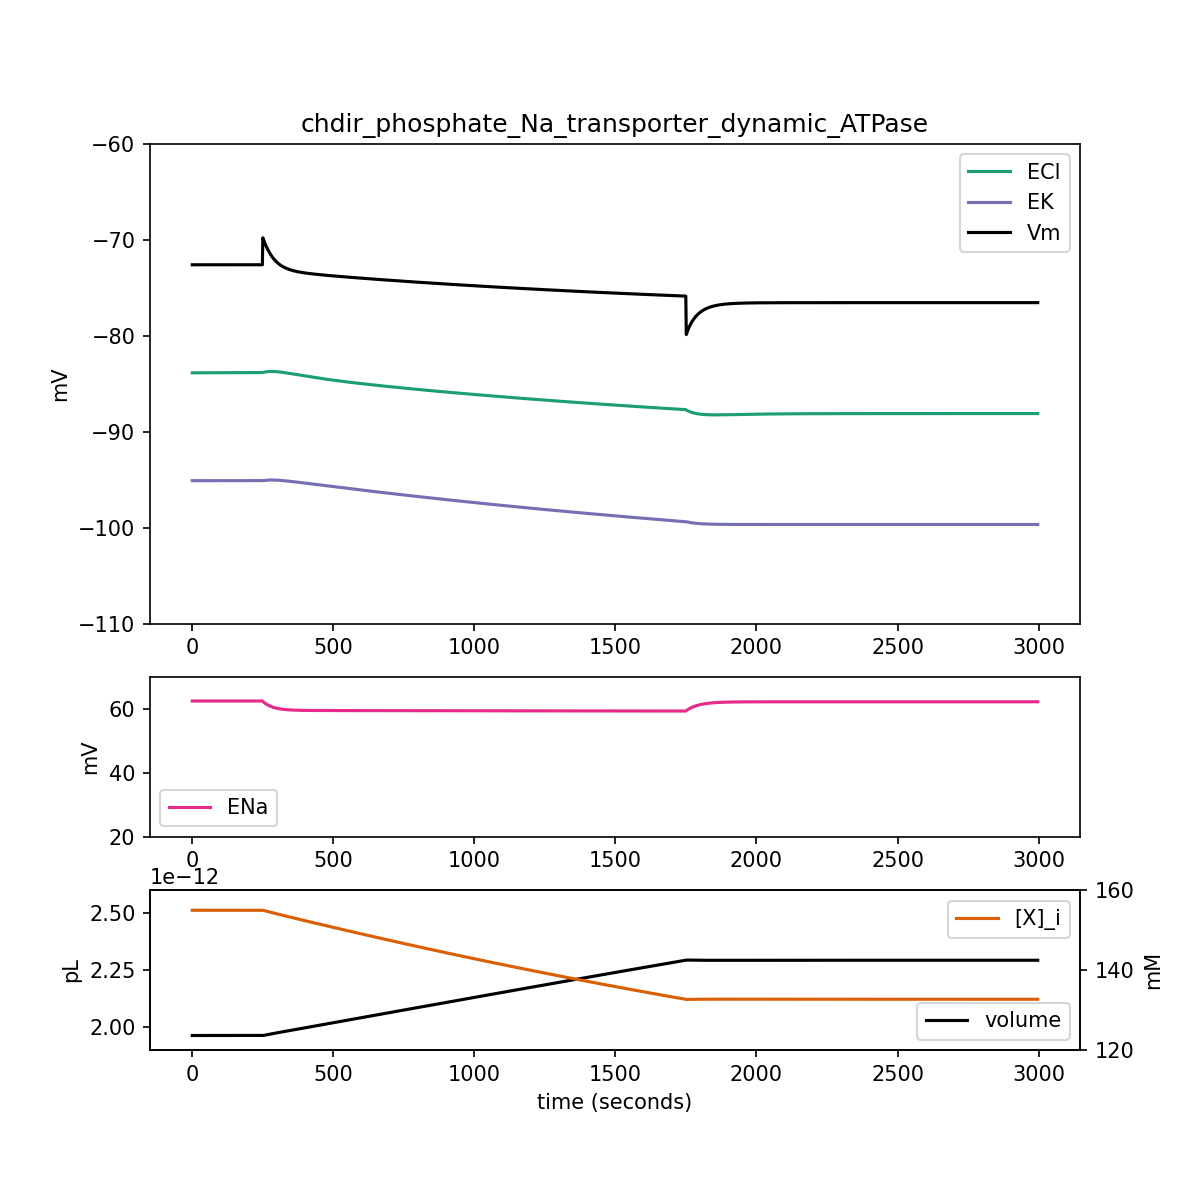
\includegraphics[width=0.5\textwidth]{images/chdir_phosphate_Na_transporter_dynamic_ATPase.png}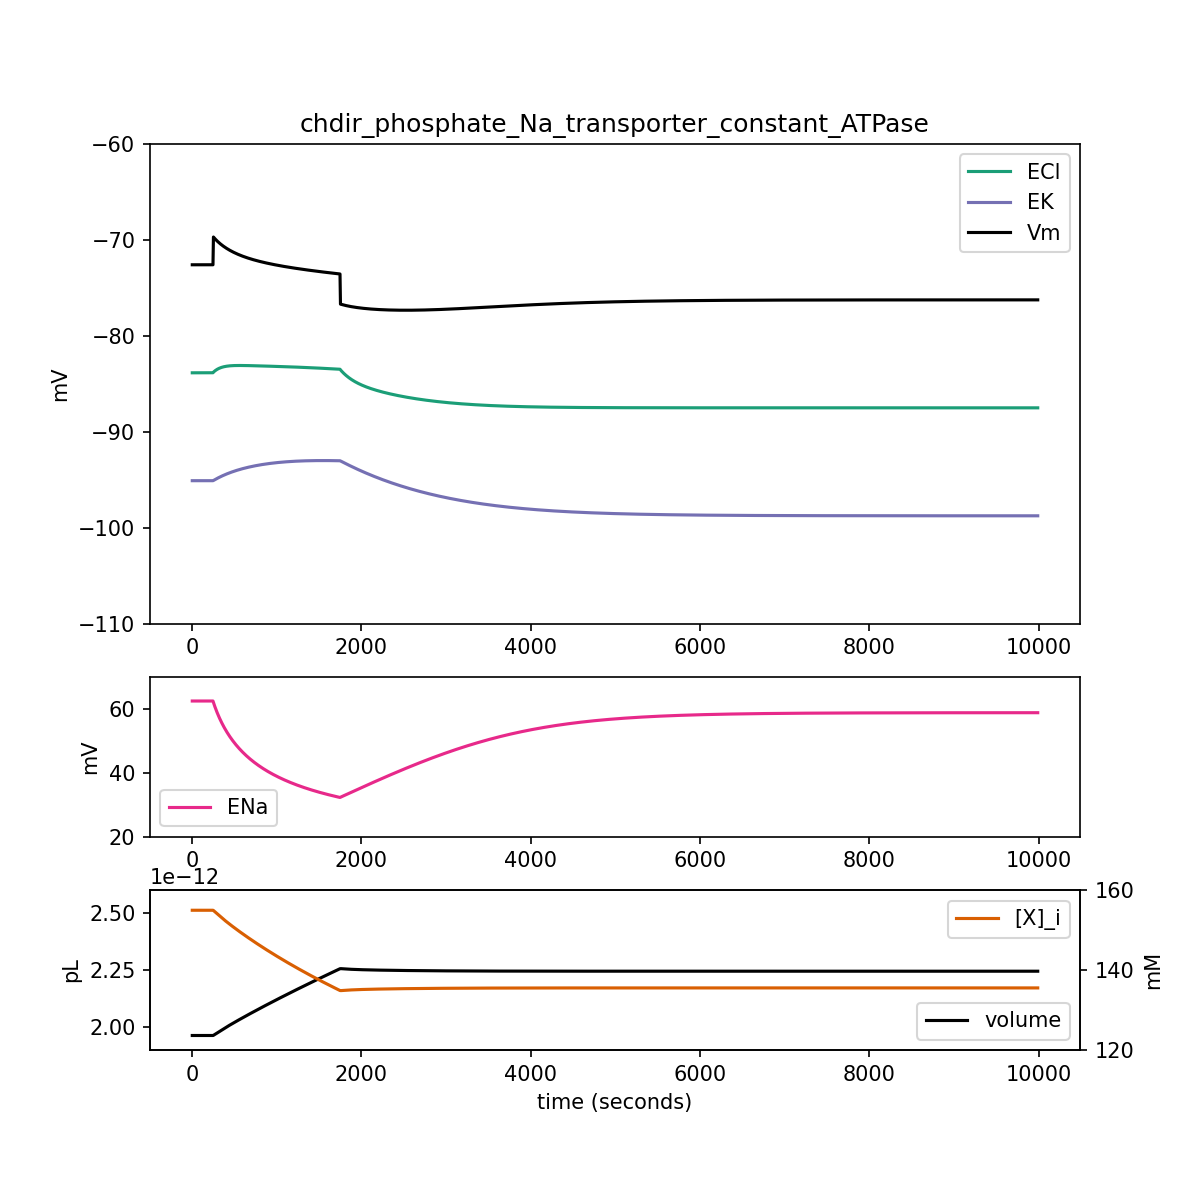
\includegraphics[width=0.5\textwidth]{images/chdir_phosphate_Na_transporter_constant_ATPase.png}
\caption{Model of Na-Pi transporter activity in the cell when phosphate is not incorporated in DNA. \textbf{A}: Using a cubic, dynamic ATPase model \cite{Dusterwald2018}, between 250 and 1750 seconds, the Na-Pi transporter is switched on. There are sustained changes in membrane potentials (top and middle). There are negligible increases in cell volume (black, bottom) for a moderate decrease in impermeant intracellular phosphate (bottom, orange). Switching off the transporter from 1750 seconds leads to new equilibria. \textbf{B}: Now substituting the ATPase rate for a constant pump rate, the dynamics of ion reversal potential shifts are altered and the change in sodium is of much greater magnitude. \label{f1}}
\end{figure}

\begin{figure}[h]
\centering A  \hskip 80mm B \\
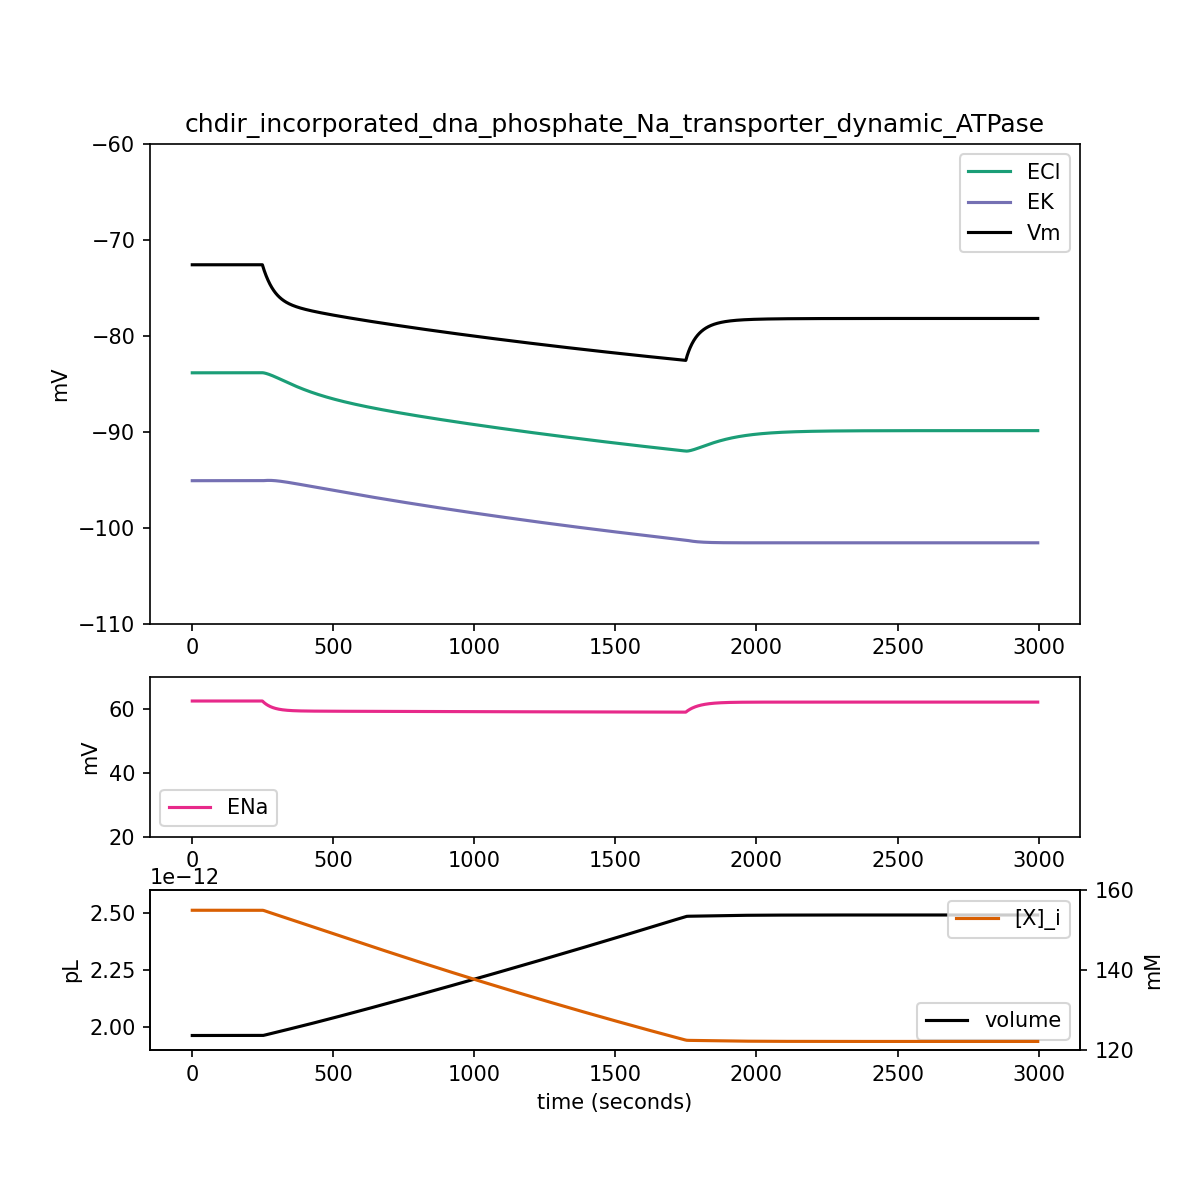
\includegraphics[width=0.5\textwidth]{images/chdir_incorporated_dna_phosphate_Na_transporter_dynamic_ATPase.png}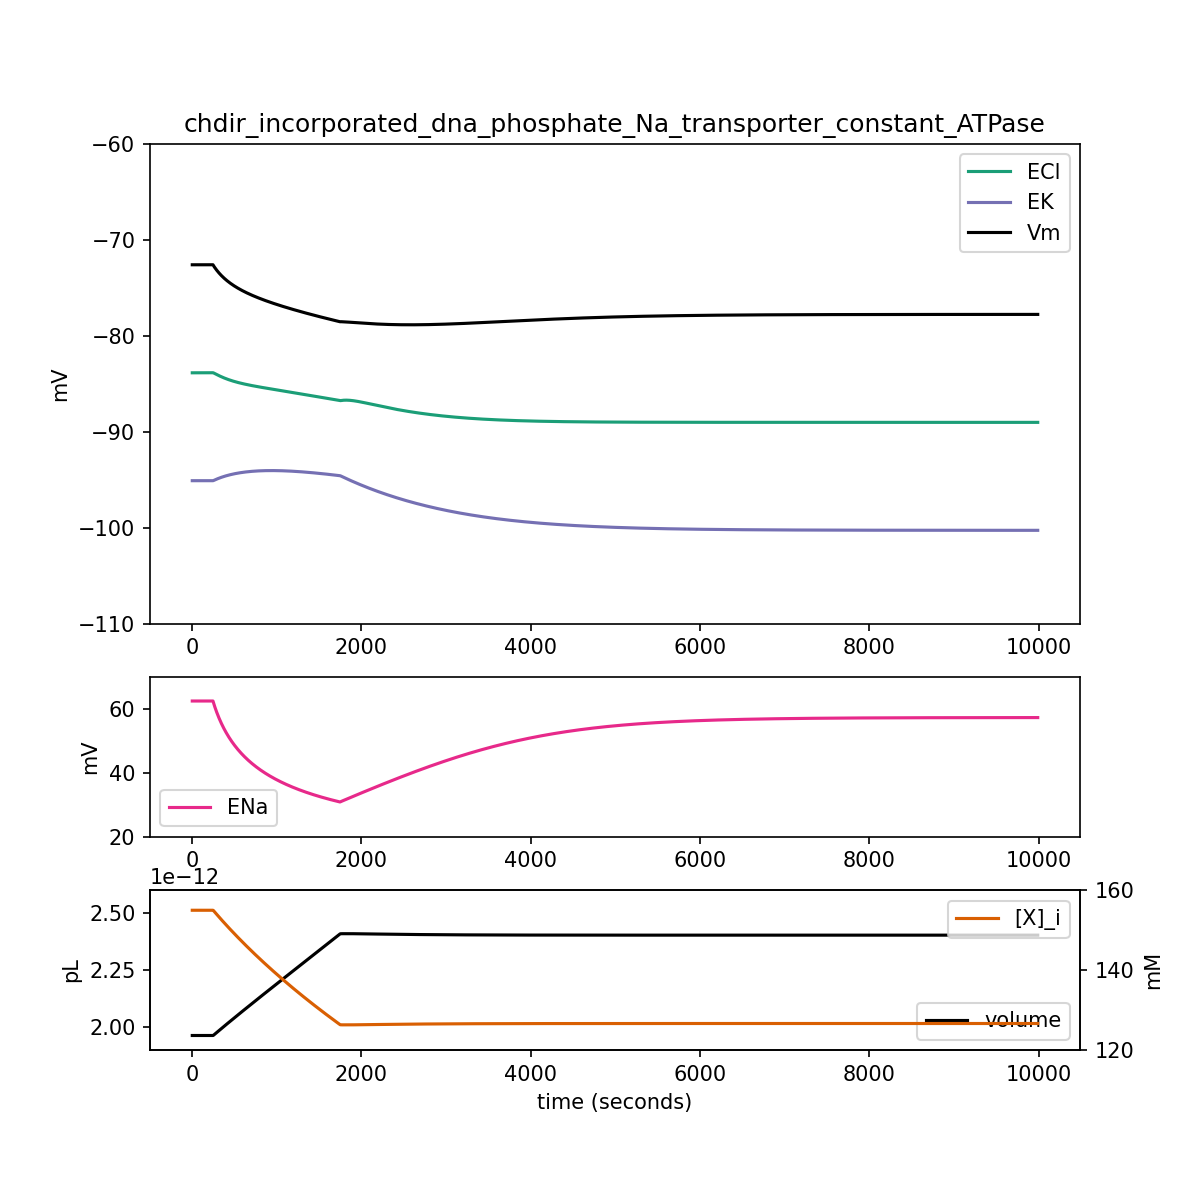
\includegraphics[width=0.5\textwidth]{images/chdir_incorporated_dna_phosphate_Na_transporter_constant_ATPase.png}
\caption{Model of Na-Pi transporter activity in the cell when phosphate is incorporated in DNA. \textbf{A}: Using a cubic, dynamic ATPase model \cite{Dusterwald2018}, between 250 and 1750 seconds, the Na-Pi transporter is switched on. There are sustained changes in membrane potentials (top and middle). There are negligible increases in cell volume (black, bottom) for a moderate decrease in impermeant intracellular phosphate (bottom, orange). Switching off the transporter from 1750 seconds leads to new equilibria. \textbf{B}: Now substituting the ATPase rate for a constant pump rate, the dynamics of ion reversal potential shifts are altered and the change in sodium is of much greater magnitude. \label{f2}}
\end{figure}

\subsection{ATPase pump form results in different dynamic shifts}
In all models, there is dynamic hyperpolarisation of the cell membrane and increase in intracellular sodium (resulting in a decrease in $E_{Na}$). The sodium concentration increase is much larger when a static ATPase pump rate is used (Fig. \ref{f1}, \ref{f2} B, middle panel), since the pump cannot increase in rate secondary to sodium accumulation. At steady state, there is also a larger sustained increase in sodium compared to the dynamic model ($\approx 20$ mM change in static, compared to $\approx 1$ mM in dynamic, see Appendix \ref{app}). Changes in potassium are similar, $\approx 30$ mM. 

The ATPase rate form is important when considering the other permeable ions during the transporter activation. For a dynamic rate (Fig. \ref{f1} A, \ref{f2} A), there are decreases in chloride and potassium. For a static ATPase rate (Fig. \ref{f1} B, \ref{f2} B), potassium increases while the transporter is active, and chloride can shift in different directions depending on the integration of phosphate in DNA. Chloride increases slightly when phosphate is not incorporated in the existing anions (Fig. \ref{f1} B, top panel) and increases when it is incorporated (Fig. \ref{f2} B, top panel).

\subsection{Effects on chloride driving force}
There are dynamic changes in chloride driving force in the model. As previously shown \cite{Dusterwald2018}, there are no sustained changes to chloride driving force when the ATPase is kept constant (Fig. \ref{f1}, \ref{f2} B, top panel), while the dynamic ATPase transporter can add energy to the system based on the sodium gradient.

\section{Conclusions and further work}

We show that a biophysical model of a selectively-active sodium-phosphate transporter can produced sustained decreases in membrane potential, and increases in potassium and sodium concentrations. Dynamics during the transporter activation differ dependent on ATPase rate, which can be dynamic or constant. Whether the phosphate is incorporated in DNA or remains a separate intracellular impermeant anion affects volume shifts and the final concentration of impermeants in the cell.

Further work should investigate the mechanisms underlying ATPase pump-rate dependence in the dynamic phase of the transporter activation, the mathematical conditions required for the Na-Pi transporter to reach steady state when active and models of other potential phosphate transport mechanisms. The relative speed and number of phosphate ions that react with and are combined in DNA could also be considered in more detail.

\bibliographystyle{ieeetr}
\bibliography{ref}

\section{Appendix: interim values for simulations \label{app}}

Here the output of interim values is presented. $Tp_{end}$ values are the values at the end of the time period for which the Na-Pi transporter is switched on. The ions' intracellular molar concentrations are given by $na, k, cl, x$, while membrane potential $vm$ is in volts, and volume $w$ is in litres. $z$ is the charge of the impermeant anions.

\begin{verbatim}
Figure 2A
Initial values: na 0.014002 k 0.122873 cl 0.005163 x 0.154962 vm -0.06874556249996833
w 1.9634954084936206e-12 radius 5e-05 z -0.85
Tp_end values: na 0.015947371677036287 k 0.15493249174941362 cl 0.0038047331819436336 
x 0.12247500898981584 vm -0.08255664893323114 deltx -3.473512337869159e-26
Final values: na 0.014181044842723771 k 0.1565582271082254 cl 0.004120566410928825 
x 0.12214016242119909 vm -0.0781865320559633 deltx -3.4785610476625737e-26
w 2.4911312500280737e-12 radius 5.631879631758194e-05 z -1.364206970747865
ecl -89.87972684903485

Figure 2B
Initial values: na 0.014002 k 0.122873 cl 0.005163 x 0.154962 vm -0.06874556249996833
w 1.9634954084936206e-12 radius 5e-05 z -0.85
Tp_end values: na 0.0456339693045345 k 0.12050491740974363 cl 0.004632354960054675 
x 0.126353538385696 vm -0.07852719354647082 deltx -2.0548248859196916e-26
Final values: na 0.016995351439206656 k 0.14911957226686332 cl 0.0042556513016178375 
x 0.1266294249433151 vm -0.07776350754730005 deltx -1.933655850877744e-26
w 2.402815740710916e-12 radius 5.5311481807896354e-05 z -1.2782582012810206
ecl -89.017652151927

Figure 1A
Initial values: na 0.014002 k 0.122873 cl 0.005163 x 0.154962 vm -0.06874556249996833
w 1.9634954084936206e-12 radius 5e-05 z -0.85
Tp_end values: na 0.015741519276248866 k 0.14420392198599502 cl 0.00447199799518736 
x 0.13267578834593188 vm -0.07585661604212533 deltx 2.5748419946413825e-27
Final values: na 0.014128621735866183 k 0.14577187586251167 cl 0.004404134146662227 
x 0.13269536842742888 vm -0.07653715244965972 deltx 6.664296927307108e-26
w 2.292975098505106e-12 radius 5.403245849033436e-05 z -1.1718738771623982
ecl -88.10109578887266

Figure 1B
Initial values: na 0.014002 k 0.122873 cl 0.005163 x 0.154962 vm -0.06874556249996833
w 1.9634954084936206e-12 radius 5e-05 z -0.85
Tp_end values: na 0.04327921003424906 k 0.11368208764625075 cl 0.005235275283488621 
x 0.13487969832448848 vm -0.07355032699199518 deltx -4.957833017133015e-26
Final values: na 0.0160541786059926 k 0.14090965828904198 cl 0.004503754103743571 
x 0.1355324089765185 vm -0.07624826081864017 deltx -1.5247103576111716e-26
w 2.2449772551721455e-12 radius 5.346394877219768e-05 z -1.1249412329839887
ecl -87.503320879327
\end{verbatim}

\end{document}